\begin{frame}{Cyclic graphs}
\label{sec:toy}
\begin{columns}
\begin{column}{0.4\textwidth}
% We now add cycles to the DAG from before~(\autoref{sec:dag}). The edges are also given randomly selected values in range $[-1,1]$~(\autoref{fig:toy}).
\begin{figure}[ht]
    \centering
    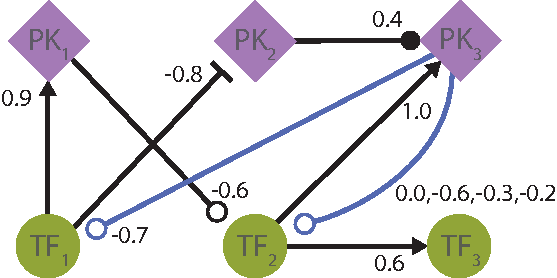
\includegraphics[width=0.7\textwidth]{analysis/fig/toy.pdf}
    \caption{\textbf{Directed cyclic networks.} \textcolor{blue}{blue} = edges added onto DAG. Multiple values: four separate graphs each assigned one of the four values. }
    \label{fig:toy}
\end{figure}
% Four separate graphs are tested to analyse the balance between predicting that an edge is present from a protein kinase to a transcription factor or that the observed effect is mediated through another protein kinase.

\vskip2\baselineskip

$\pk_2\rightarrow\pk_3$ is favored over $\pk_2\rightarrow\tf_{}$ when increasing $\pk_3\rightarrow\tf_{}$
\end{column}

\begin{column}{0.6\textwidth}
\begin{figure}[ht]
\centering
\begin{subfigure}[b]{0.4\textwidth}\centering\caption{}
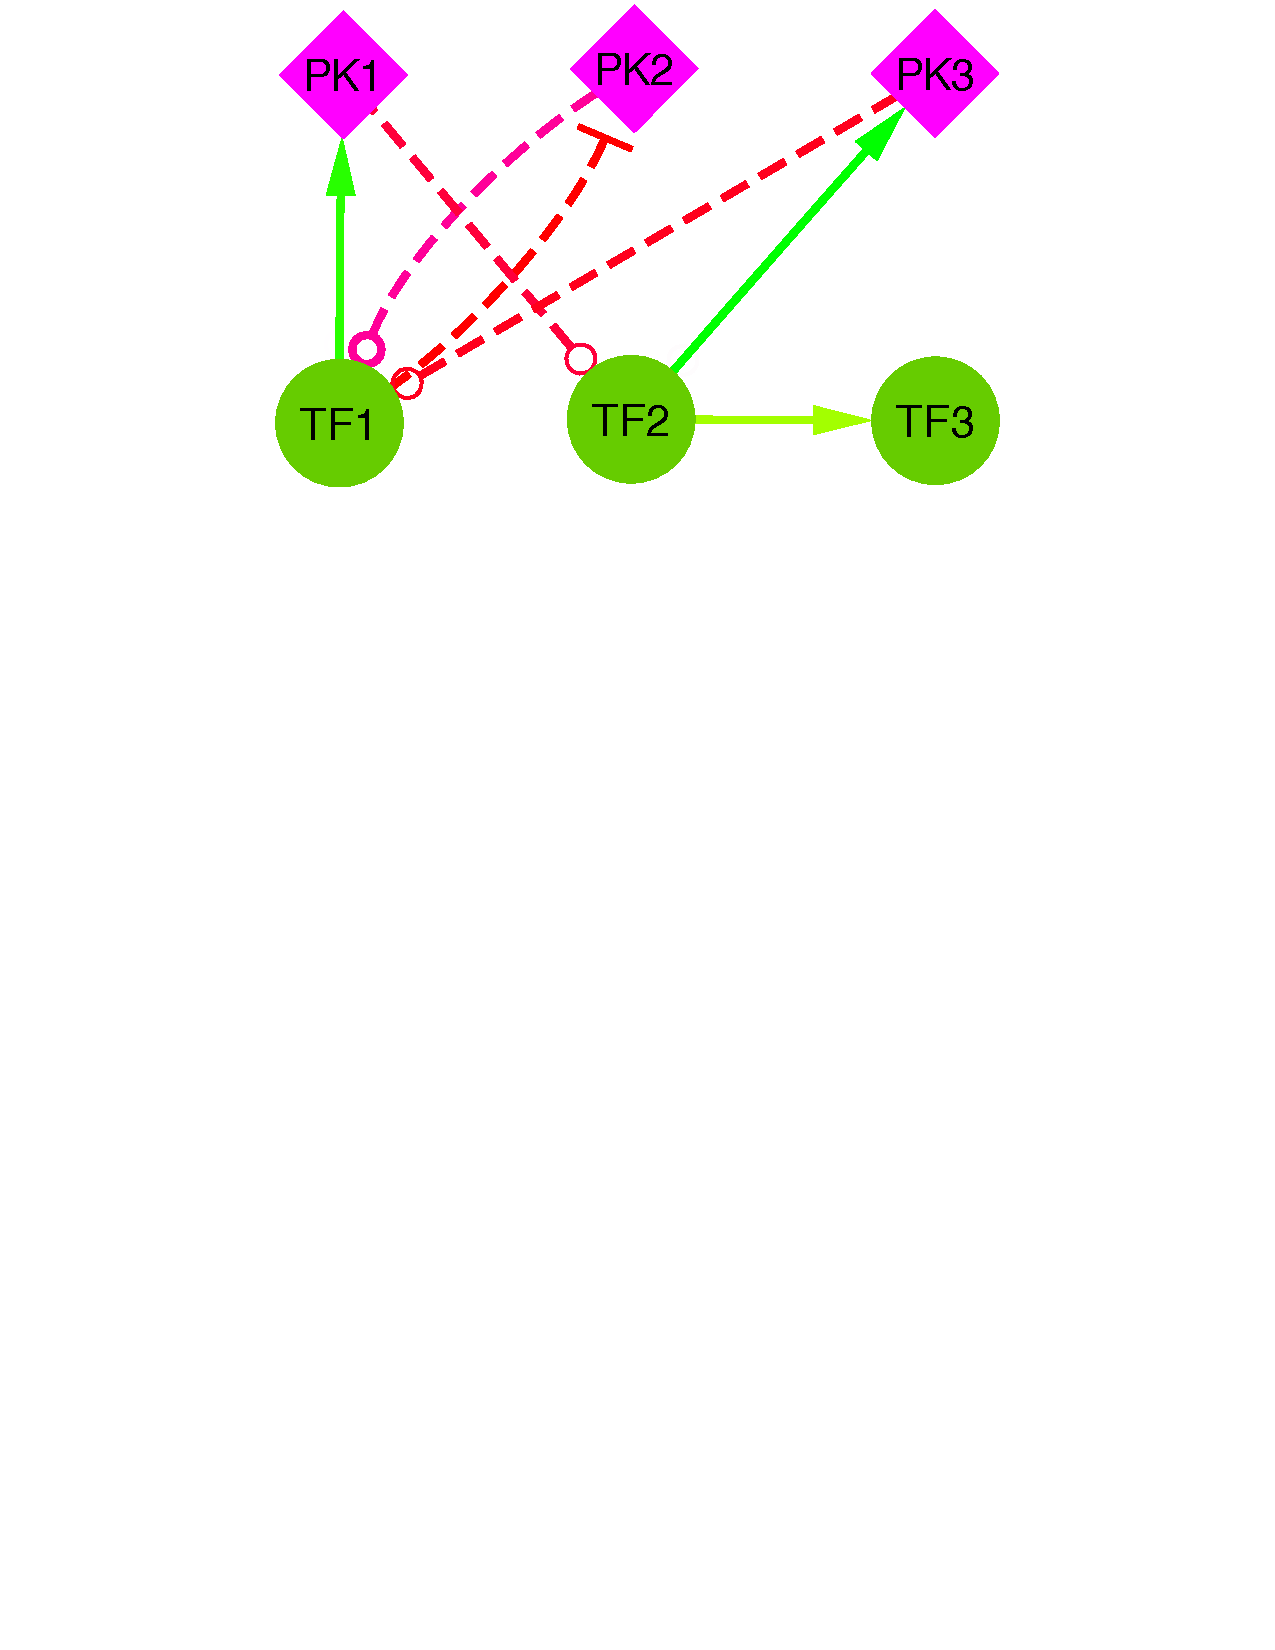
\includegraphics[width=0.8\textwidth]{analysis/fig/cyclic_2.pdf}\label{fig:toy_infer.a}
\end{subfigure}
\quad
\begin{subfigure}[b]{0.4\textwidth}\centering\caption{}
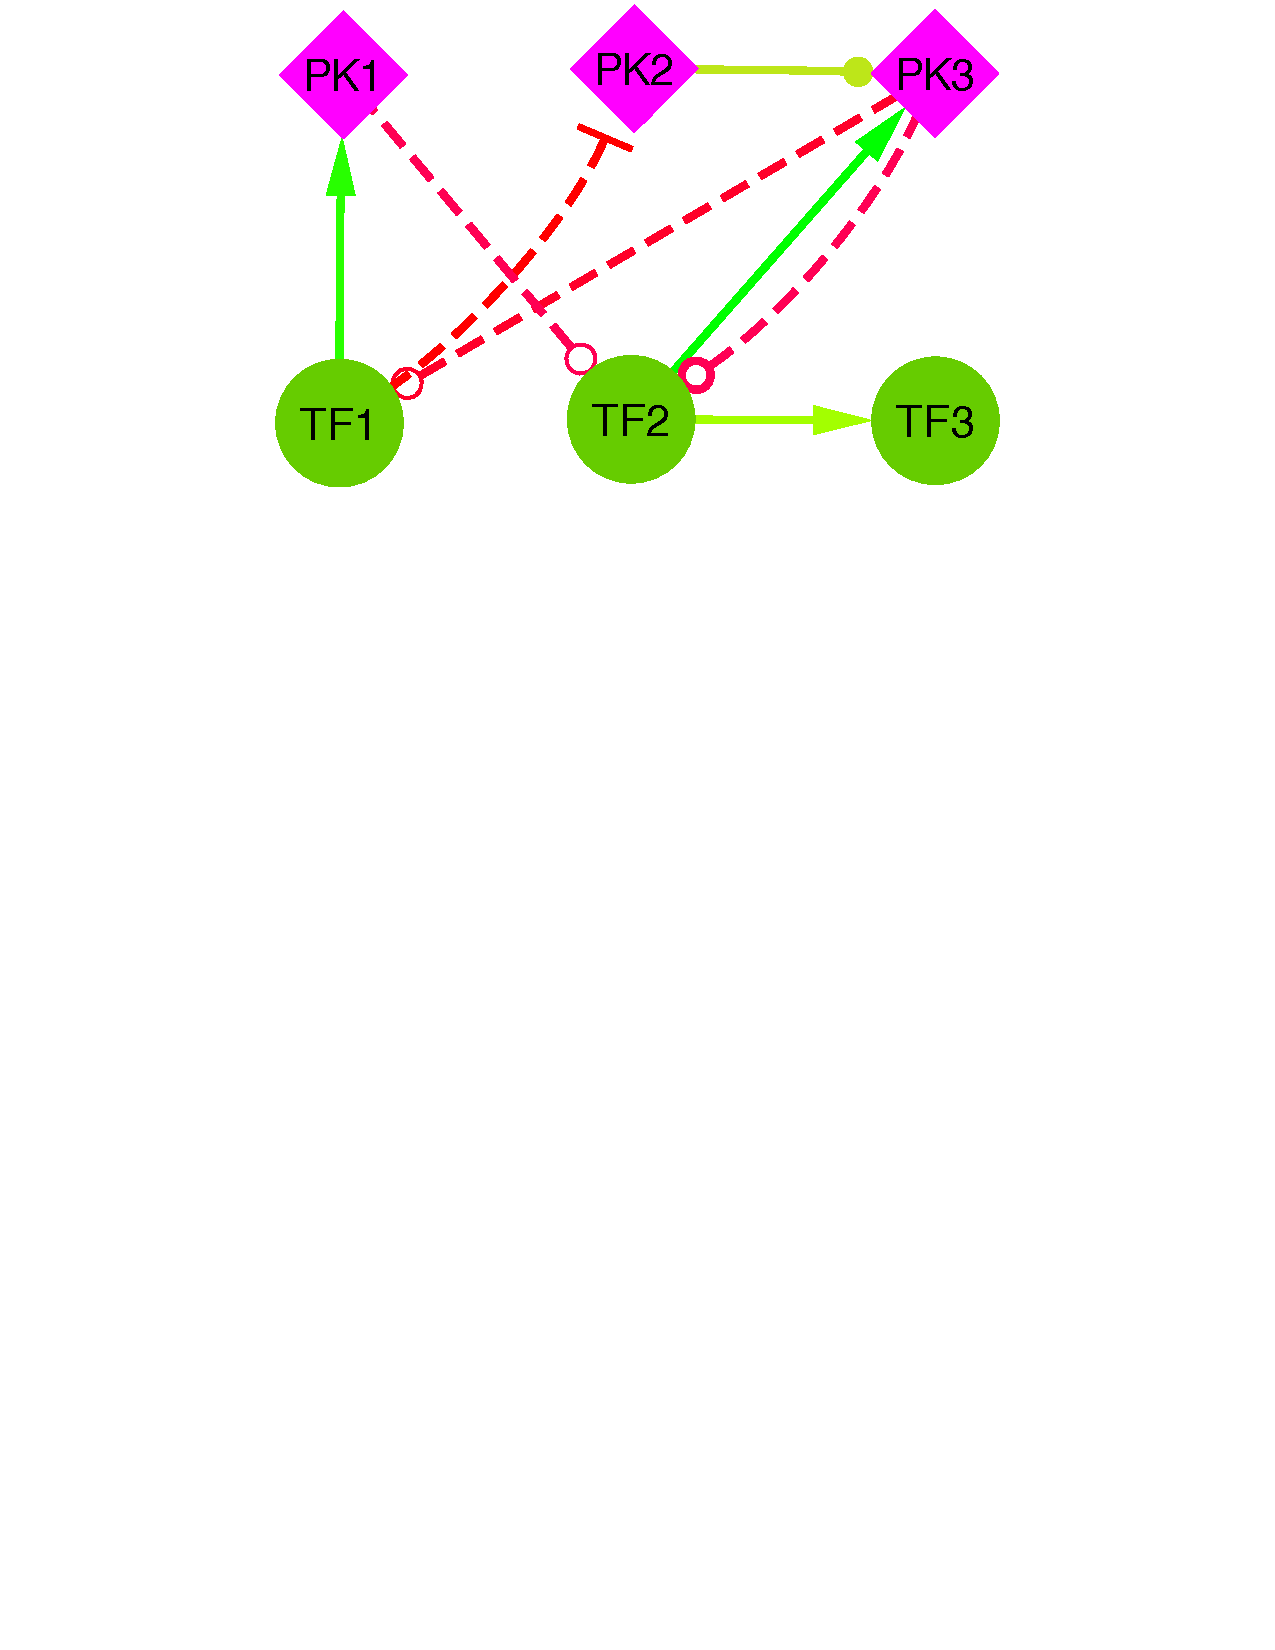
\includegraphics[width=0.8\textwidth]{analysis/fig/cyclic_3.pdf}\label{fig:toy_infer.b}
\end{subfigure}
\vskip\baselineskip
\begin{subfigure}[b]{0.4\textwidth}\centering\caption{}
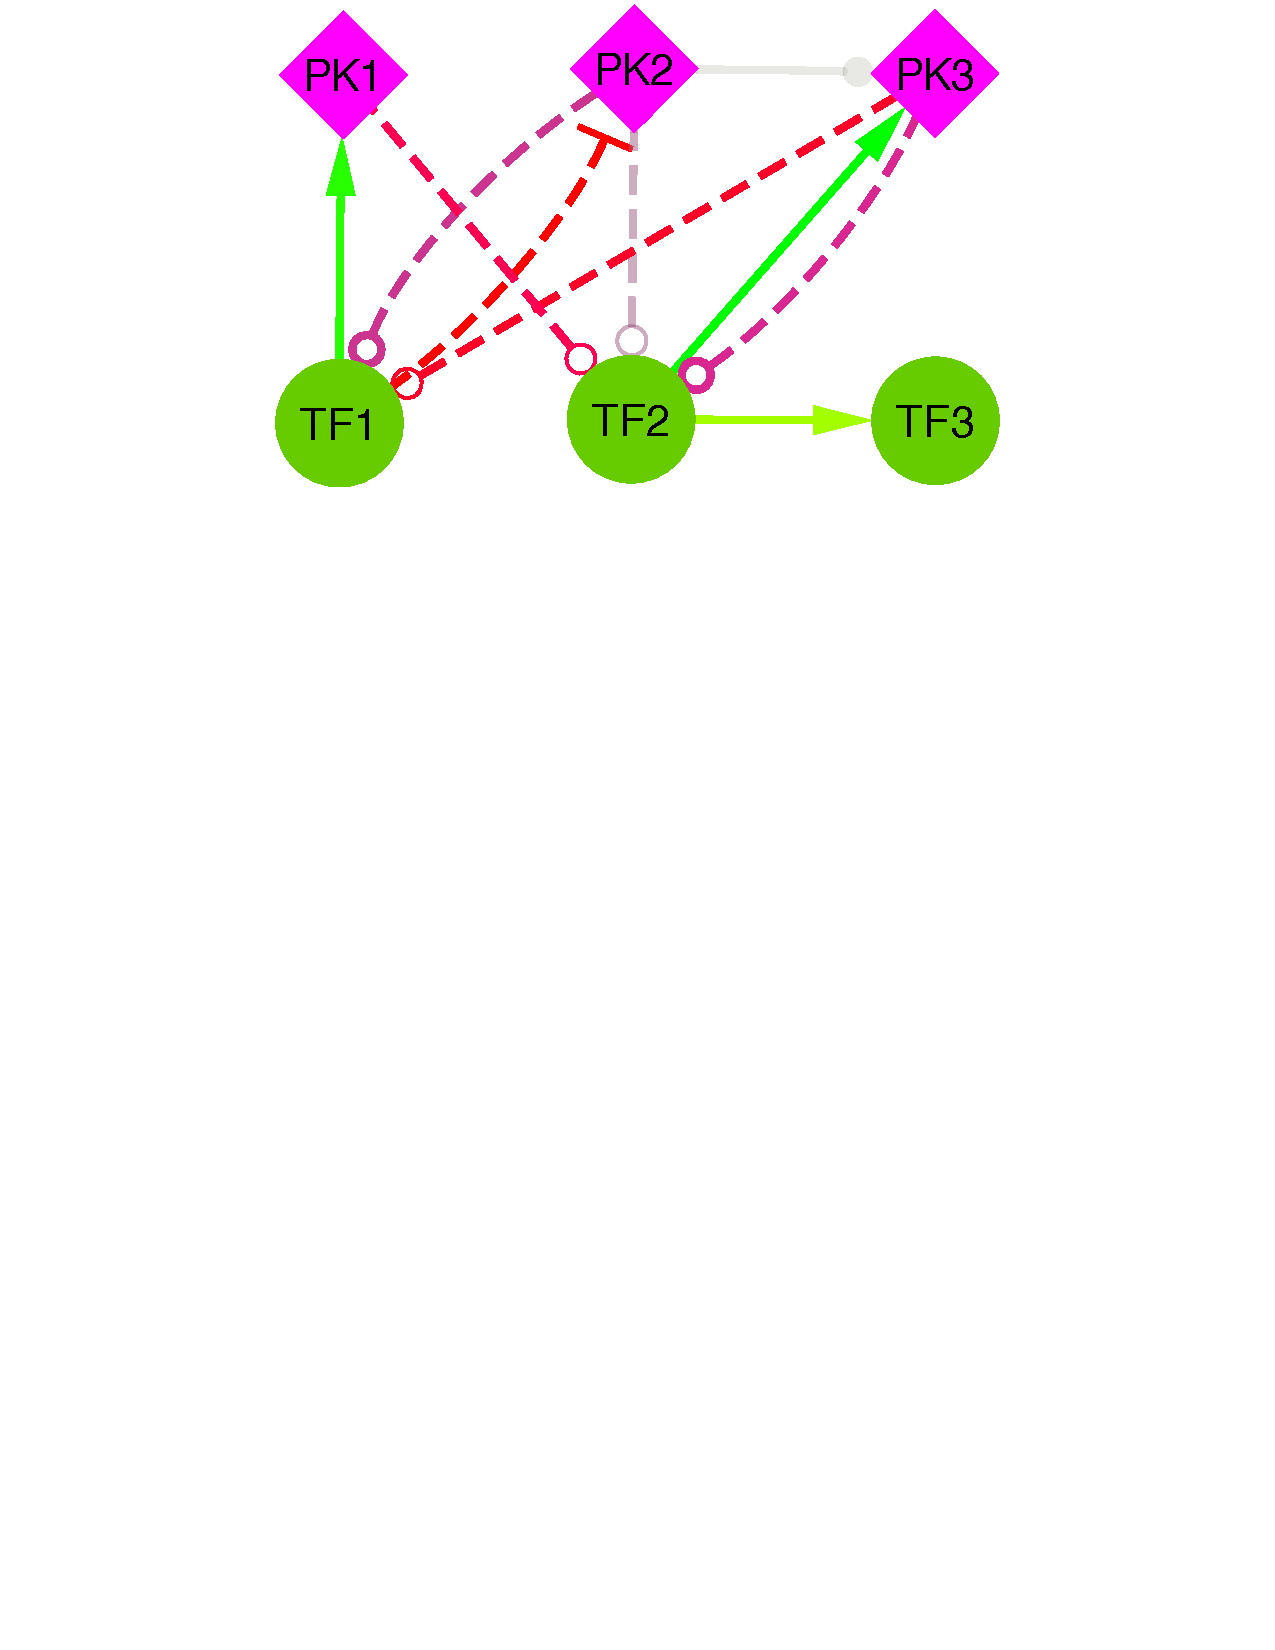
\includegraphics[width=0.8\textwidth]{analysis/fig/cyclic_4.pdf}\label{fig:toy_infer.c}
\end{subfigure}
\quad
\begin{subfigure}[b]{0.4\textwidth}\centering\caption{}
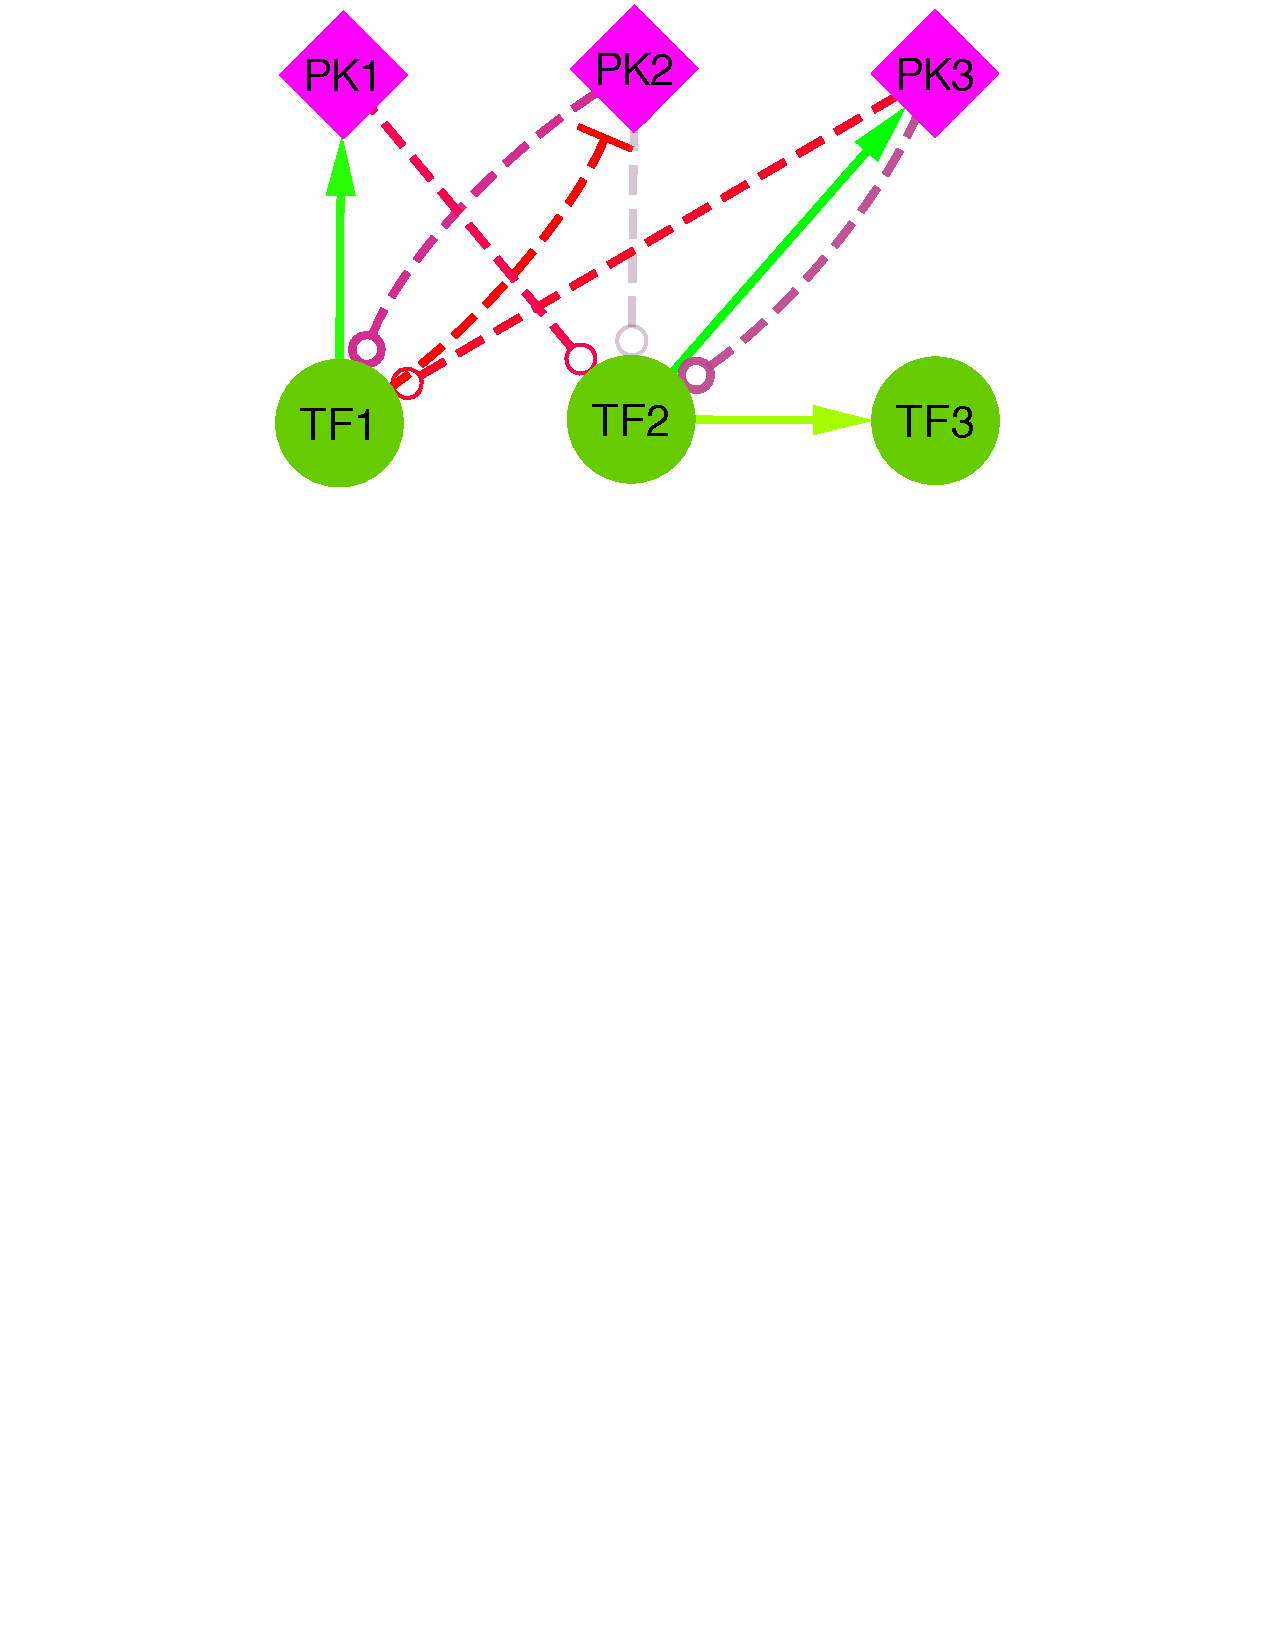
\includegraphics[width=0.8\textwidth]{analysis/fig/cyclic_5.pdf}\label{fig:toy_infer.d}
\end{subfigure}
\vskip\baselineskip
\begin{subfigure}[b]{0.3\textwidth}\centering
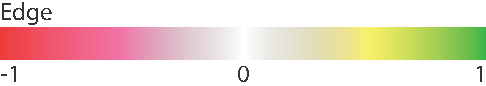
\includegraphics[width=\textwidth]{analysis/fig/edge_legend_cyclic.pdf}
\end{subfigure}
\caption{\textbf{Edge inference.} True $\pk_3\rightarrow\tf_2$ = 0~(\text{a}), -0.6~(\text{b}), -0.3~(c), -0.2~(d). $\boldsymbol{e}$-minimization~($\lambda_T=0.01, \lambda_P=0.01$). Simple simulation. }
\label{fig:toy_infer}
\end{figure}

% Node values were simulated on each of the four graphs with approximate convergence using the simple iterative approach~(\autoref{sec:prim}). Edge values were then inferred using the $\boldsymbol{e}$-minimization method with $\lambda_{TF} = 0.01$ and $\lambda_{PK} = 0.01$~(\autoref{sec:equilibrium_model}). The inferred edges are shown in~\autoref{fig:toy_infer} for each of the four graphs produced from varying a single edge value as indicated in~\autoref{fig:toy}.

% First, the leftmost blue edge in~\autoref{fig:toy} is added to the DAG~(the rightmost blue edge has an edge value of zero). We observe that the inference method now detects the effect of $\pk_2$, but it predicts it is a direct edge to $\tf_1$, rather than an indirect effect mediated by $\pk_3$~(\autoref{fig:toy_infer.a}). This is a rational prediction, given that the node value data would be equivalent in a case where an edge from $\pk_2$ to $\tf_1$ was present, with edge value equal to the product of the true edge values from $\pk_2\rightarrow \pk_3$ and $\pk_3\rightarrow \tf_1$.
\end{column}
\end{columns}
\end{frame}

\begin{frame}{Cyclic graphs - favoring PK$\rightarrow$PK vs. PK$\rightarrow$TF}

% Next, we show that if $\pk_3$ were to have more outgoing edges, in this case directly to $\tf_2$, then the inference will predict the $\pk_2\rightarrow \pk_3$ edge correctly~(\autoref{fig:toy_infer.b}). Even though it is still possible to explain the observed effect from $\pk_2$ to $\tf_1$ and $\tf_2$, it is the favored explanation, that the effect is mediated by a single edge from the protein kinase: $\pk_2 \rightarrow \pk_3$ (option A), rather than needing two edges: $\pk_2 \rightarrow \tf_1$ and $\pk_2 \rightarrow \tf_2$ (option B). This is a result of regularization, where by applying an L1-regularization to all parameters~(edge values), we predict the parameters that explains the data with the smallest possible edge values, which reduces the count of edges and promotes sparsity. 

% The balance between the choice of a PK$\rightarrow$TF edge versus a PK$\rightarrow$PK$\rightarrow$TF path, is based on the smallest sum of absolute edge values for each case. We explore this by reducing the edge value for the rightmost blue edge in~\autoref{fig:toy}. We observe that for small values, option B with two edges, $\pk_2 \rightarrow \tf_1$ and $\pk_2 \rightarrow \tf_2$, will be favorable~(\autoref{fig:toy_infer.d}), and for a certain threshold both option A and B will be equally likely, at which point all paths are inferred to have a combined effect~(\autoref{fig:toy_infer.c}). The threshold is found when the L1-regularization are the same for option A and B, given that $\boldsymbol{e}$ is equal for both options~(\autoref{eq:loss_e}). We formulate the L1-norm cost for all paths from $\pk_2$ in option A and B:
Option A: $\pk_{}\rightarrow\pk_{}$ \\
Option B: $\pk_{}\rightarrow\tf_{}$ \\
Norms differentiating loss for option A and B
\begin{subequations}
\label{eq:toy_l1}
\begin{align}
L1_{\pk_2\rightarrow\pk_3}
&=
|w_{\pk_2\rightarrow\pk_3}^{(\text{A})}|
\\
L1_{\pk_2\rightarrow \{\tf_1,\tf_2\}}
&=
|w_{\pk_2\rightarrow \tf_1}^{(\text{B})}| + |w_{\pk_2\rightarrow \tf_2}^{(\text{B})}|
\label{eq:toy_l1.B}
\end{align}
\end{subequations}


% Superscripts $(\text{A})$ and $(\text{B})$ indicates the option, where a weight parameters $w^{(\text{A})}$ will be nonzero for option A and $w^{(\text{B})}$ nonzero for option B. If the effects from $\pk_2$ to both $\tf_1$ and $\tf_2$ are perfectly captured for option A and B, then the total effects can be written using notation similar to~\autoref{sec:eberhardt}:

Effects from $\pk_2$ to \textcolor{tf}{TFs} are equal for choice A and B
\begin{subequations}
\label{eq:toy_t}
\begin{align}
t(\pk_2 \rightsquigarrow \tf_1)
&=
w_{\pk_2\rightarrow \pk_3}^{(\text{A})} \cdot
t(\pk_3 \rightsquigarrow \tf_1)
=
w_{\pk_2\rightarrow \pk_3}^{(\text{A})} \cdot 
w_{\pk_3\rightarrow \tf_1}
\\
&=
w_{\pk_2\rightarrow \tf_1}^{(\text{B})}
\\
t(\pk_2 \rightsquigarrow \tf_2)
&=
w_{\pk_2\rightarrow \pk_3}^{(\text{A})} \cdot t(\pk_3 \rightsquigarrow \tf_2)
=
w_{\pk_2\rightarrow \pk_3}^{(\text{A})} \cdot w_{\pk_3\rightarrow \tf_2}
\\
&=
w_{\pk_2\rightarrow \tf_2}^{(\text{B})}
\end{align}
\end{subequations}

\end{frame}
\begin{frame}{Cyclic graphs - favoring PK$\rightarrow$PK vs. PK$\rightarrow$TF}


% By summing~\autoref{eq:toy_t} we can formulate $L1_{\pk_2 \rightarrow \pk_3}$:

\begin{subequations}
\begin{align}
|t(\pk_2 \rightsquigarrow \tf_1)| + |t(\pk_2 \rightsquigarrow \tf_2)| &=
|w_{\pk_2\rightarrow \pk_3}^{(\text{A})}|
\left(|w_{\pk_3\rightarrow \tf_1}| + |w_{\pk_3\rightarrow \tf_2}|\right)
\\
&= |w_{\pk_2\rightarrow \tf_1}^{(\text{B})}| + |w_{\pk_2\rightarrow \tf_2}^{(\text{B})}|
\\
\implies
L1_{\pk_2 \rightarrow \pk_3}
&=
\frac
{|w_{\pk_2\rightarrow \tf_1}^{(\text{B})}| + |w_{\pk_2\rightarrow \tf_2}^{(\text{B})}|}
{|w_{\pk_3\rightarrow \tf_1}| + |w_{\pk_3\rightarrow \tf_2}|}
\\
&=
\frac{
L1_{\pk_2\rightarrow\{\tf_1,\tf_2\}}
}{
|w_{\pk_3\rightarrow\tf_1}| + |w_{\pk_3\rightarrow \tf_2}|
}
\end{align}
\end{subequations}

% This means that option A has the lowest L1-norm, and is inferred, when edges from $\pk_3$ sum to more than 1, option B is inferred when they sum to less than 1, and both options are combined when edges from $\pk_3$ sum to 1. It is demonstrated in~\autoref{fig:toy_infer.b}, \ref{fig:toy_infer.c}, and \ref{fig:toy_infer.d}, where the sums are $|-0.7| + |-0.6| = 1.2$, $|-0.7| + |-0.3| = 1.0$, and $|-0.7| + |-0.2| = 0.9$.

Option A favored when $|w_{\pk_3\rightarrow \tf_1}| + |w_{\pk_3\rightarrow \tf_2}| < 1$

General formulations (more norms may be compared):

% So, if the data can be perfectly modeled in either case considered, then for an edge $\text{PK}_j \rightarrow \text{PK}_i$ and for the case of direct edges from $\text{PK}_j$ to each regulated $\text{TF}_k$ the generalized L1-norms will be

\begin{subequations}
\begin{align}
L1_{\text{PK}_j \rightarrow \text{PK}_i}
&=
\frac{
L1_{\text{PK}_j \rightarrow \{\text{TF}_k\}}
}{
\sum_k |t(\text{PK}_i \rightsquigarrow \text{TF}_k)|
}
\\
L1_{\text{PK}_j \rightarrow \{\text{TF}_k\}}
&=
\sum_k |w_{\text{PK}_j \rightarrow \text{TF}_k}|
\end{align}
\end{subequations}

% Where $k$ indexes all TFs that are regulated by $\text{PK}_j$ through a directed path of PKs.

% For a more complicated graph, there can be many other L1-norms that the model will compare, than the two exemplified here.
% In general, applying the L1-regularization indiscriminately on each parameter will make the model favor paths with fewer edges. The smaller the parameters found for a dataset, the rarer PK$\rightarrow$PK edges will be inferred. The parameters will usually be less than 1 since parameters above 1 easily leads to divergence in the model.
\end{frame}
\begin{frame}{Loss function favoring longer cascades}
\label{sec:cascade_loss}
\begin{columns}
\begin{column}{0.65\textwidth}

% Other loss functions can be considered to treat longer cascades more favorably. One idea would be to replace the use of the regularization hyperparameter $\lambda_{PK}$ with a regularization strength for $\text{PK}\rightarrow\text{TF}$ and a smaller one for $\text{PK}\rightarrow\text{PK}$ edges, however this creates loops among the PKs to artificially strengthen the $\text{PK}\rightarrow\text{TF}$ edges~(not shown).

% A solution to consider is replacing the L1-regularization of PK edges with a loss based on a sum of effects $t(\text{PK}_j\rightsquigarrow\text{TF}_i)$ that each PK has through all its cascades. This is done in a similar fashion to the classification of detectable nodes~(\autoref{sec:unobservable}). 

PK edge norm = total effect on TFs
\begin{equation}
\label{eq:pk_effect}
\boldsymbol{l}_{\text{cas}} =
\sum_{k=1}^K {(|W|I_P)^\trans}^k
(I_T \boldsymbol{1} )
\end{equation}

% Here, $|W|$ is used for indication of element-wise absolute values of $W$. $K$ can be found similarly to described in~\autoref{sec:unobservable}, however due to noise in the weights while training it is best to have an upper bound for $K$, which can be chosen conservatively since the only downside to using a too large $K$ is computational cost. $W$ has to be square. If there are more measured genes than knockouts, we use $I_SW$ instead, where $I_S$ is an identity matrix with dimensions $(N_T + N_P) \times N$, and $N$ is the total number of measured genes.

% If $I-(|W|I_P)^\trans$ is invertible, we can get rid of $K$ from~\autoref{eq:pk_effect}, as it was done in~\autoref{sec:unobservable}.
for $K\rightarrow\infty$
\begin{equation}
\boldsymbol{l}_{\text{cas}} =
\left(
\sum_{k=1}^\infty {(|W|I_P)^\trans}^k
\right)
(I_T \boldsymbol{1} )
=
\left(
I-(|W|I_P)^\trans
\right)^{-1}
(I_T \boldsymbol{1} )
\end{equation}

% We define a new loss function that favors longer cascades:

\begin{equation}
\mathcal{L}_\text{cas} =
\sum_{i=1}^N e_i^2 + \lambda_T \sum_{j \in \text{TF}} \sum_{i=1}^N |w_{ij}| + \lambda_P \sum_{i=0}^{N_T + N_P} \left(
\sum_{j \in \text{PK}} |w_{ij}|
+ l_i^{(\text{cas})}
\right)
\label{eq:loss_cas}
\end{equation}

% Here, $\boldsymbol{l}_{\text{cas}}$ and the L1-norm regularization term used in~\autoref{eq:loss_e} are summed, where  $l_i^{(\text{cas})}$ is the $i$-th element of $\boldsymbol{l}_\text{cas}$.

\end{column}
\begin{column}{0.35\textwidth}
\begin{figure}[ht]
\centering
\begin{subfigure}[b]{0.7\textwidth}\centering
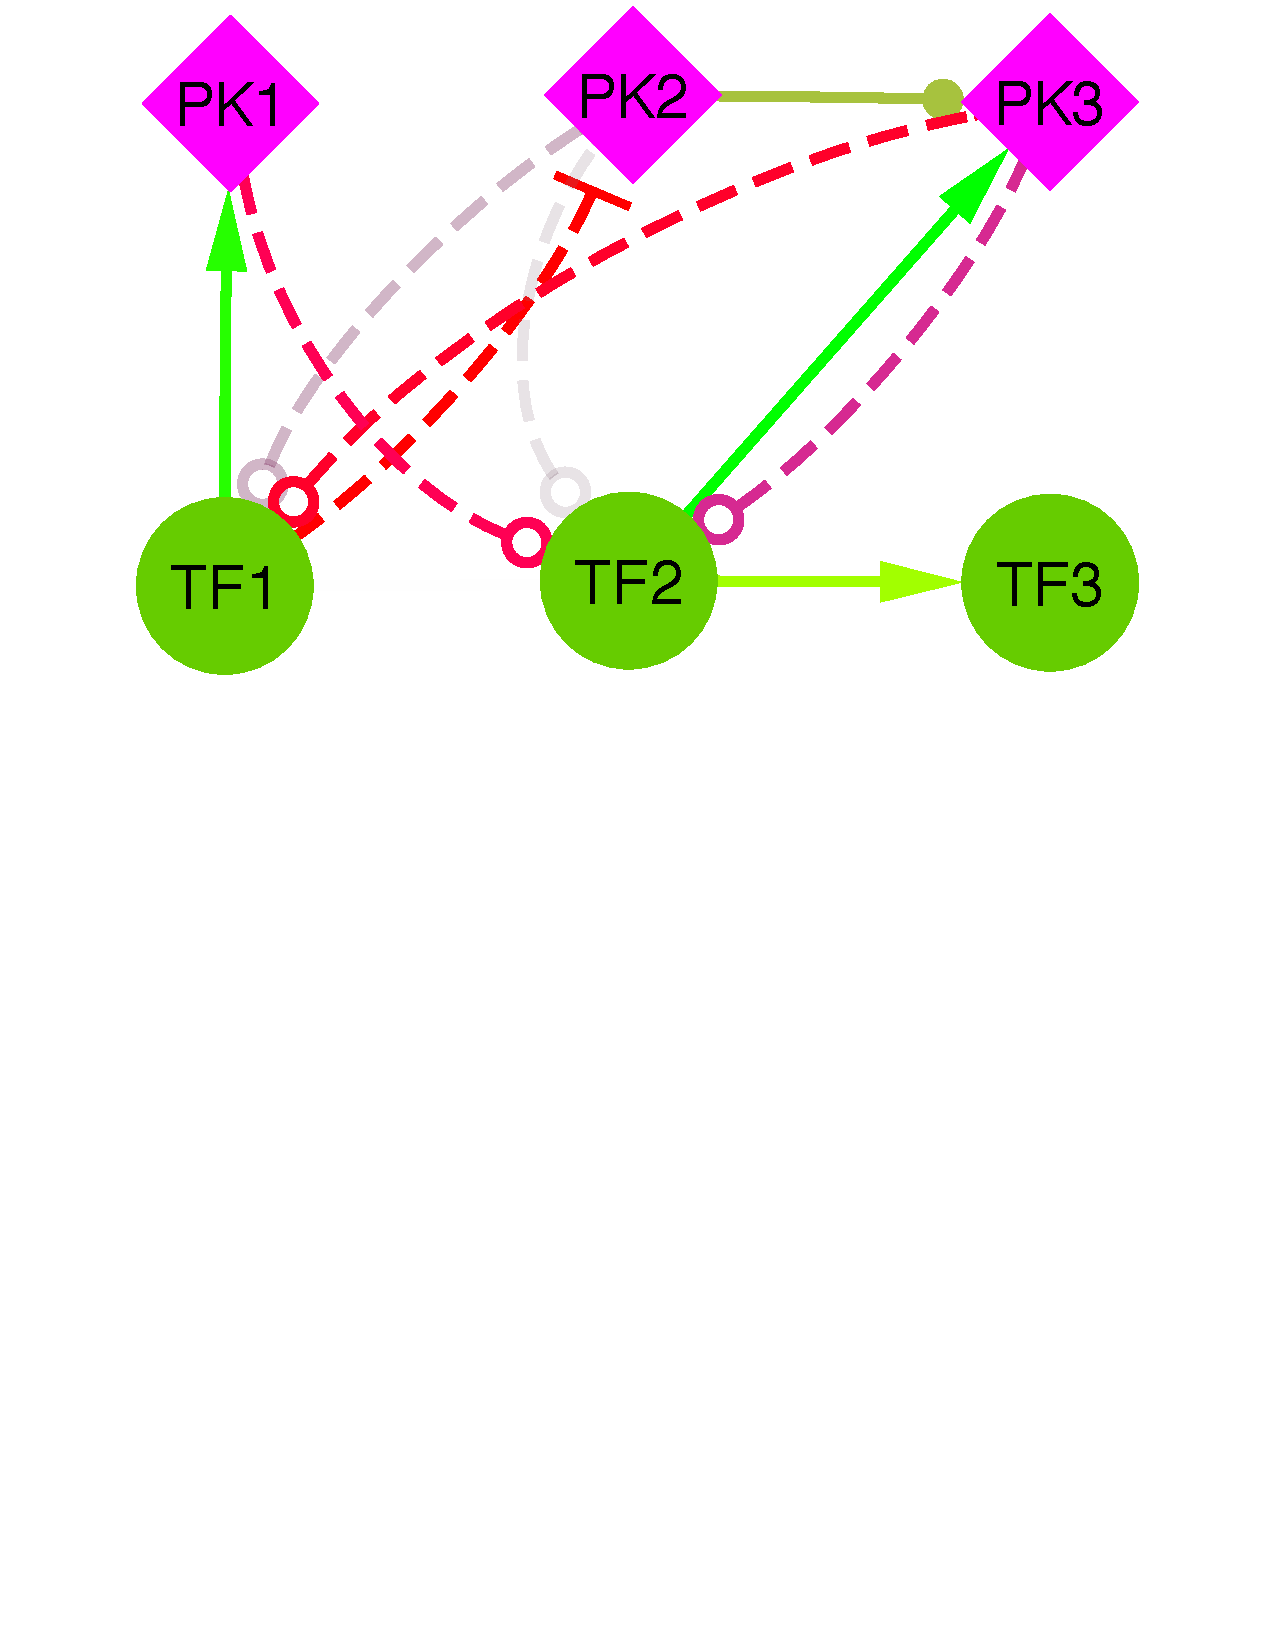
\includegraphics[width=\textwidth]{analysis/fig/cyclic_4_cas.pdf}
\end{subfigure}
\vskip\baselineskip
\begin{subfigure}[b]{0.5\textwidth}\centering
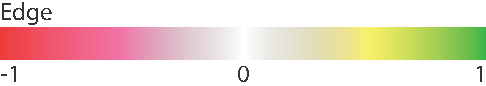
\includegraphics[width=\textwidth]{analysis/fig/edge_legend_cyclic.pdf}
\end{subfigure}
\caption{\textbf{Correcting inference.} Inference from~fig.~\ref{fig:toy_infer.c} using $\mathcal{L}_\text{cas}$~(eq.~\ref{eq:loss_cas}) instead of $\mathcal{L}_{\boldsymbol{e}}$~(eq.~\ref{eq:loss_e}).
$\lambda_T=0.01$, $\lambda_P=0.01$. }
\label{fig:toy_cas}
\end{figure}

% The loss function was tested for edge inference otherwise identical to the procedure for~\autoref{fig:toy_infer.c}, for instance instance by using $\lambda_T=0.01$ and $\lambda_P=0.01$ as before. The inferred edge values are shown in~\autoref{fig:toy_cas}. We see that the change in loss function has corrected the inference to favor the $\pk_2\rightarrow\pk_3$ edge, which has been referred to as option A.

% The remaining work in this section describes inference attempts using standard L1-regularization. $\mathcal{L}_\text{cas}$ has yet to be tested for possibilities of improving performance on larger networks.
\end{column}
\end{columns}
\end{frame}
